\documentclass[12pt, a4paper]{article}

\usepackage[utf8]{inputenc}
\usepackage[T1]{fontenc}
\usepackage[french]{babel}
\usepackage{amsmath, amssymb, amsthm}
\usepackage{graphicx}
\usepackage{booktabs}
\usepackage{siunitx}
\usepackage[hidelinks]{hyperref}
\usepackage{geometry}
\usepackage[version=4]{mhchem}
\usepackage{eurosym}
\usepackage{fancyhdr}
\usepackage{float}
\usepackage{array}
\usepackage{xcolor}

\geometry{margin=2.5cm}
\setlength{\headheight}{14.5pt}
\setlength{\emergencystretch}{3em}

\pagestyle{fancy}
\fancyhf{}
\lhead{Projet 3R - Master MECEN}
\rhead{Courtin, Richer, Ahanhanzo Glele}
\cfoot{\thepage}

\title{\textbf{Déterminants Physiques et Réglementaires des Émissions Automobiles} \\ \large Analyse de l'impact de la masse et des limites de l'homologation}
\author{Ludovic Courtin \and Mathéo Richer \and Marc Ahanhanzo Glele}
\date{Année Universitaire 2025-2026}

\begin{document}

\maketitle

\begin{abstract}
Ce rapport propose une analyse multidimensionnelle des facteurs influençant les émissions polluantes du parc automobile français. En croisant les lois de la thermodynamique, le cadre juridique européen (Règlement 2019/631) et les données de la littérature économétrique récente, nous démontrons que la masse des véhicules constitue la variable pivot de la pollution. Nous mettons en exergue le paradoxe de la "vision tunnel" du \ce{CO2} qui occulte les enjeux sanitaires des oxydes d'azote et des particules fines, tout en analysant les stratégies de contournement réglementaire telles que le \textit{pooling}. Ces fondements théoriques et réglementaires servent de socle à l'analyse empirique conduite dans la seconde partie du rapport, fondée sur les données de certification ADEME.
\end{abstract}

\tableofcontents
\newpage

% ============================================================
\section[Introduction : L'Automobile face à l'Urgence Climatique]{Introduction : L'Automobile face à la\\Urgence Climatique et Sanitaire}
% ============================================================

\subsection{Le contexte sociopolitique : de la liberté à la contrainte}

L'automobile a longtemps été le symbole de la liberté individuelle et du dynamisme économique. Cependant, l'entrée dans l'anthropocène et les rapports successifs du GIEC ont déplacé le curseur vers une nécessité de régulation stricte. En France, le secteur des transports est le premier émetteur de gaz à effet de serre (GES), représentant près de \SI{31}{\percent} des émissions nationales, et le seul secteur dont les émissions n'ont pas significativement décliné depuis 1990. Ce constat contraste avec les ambitions affichées par l'Accord de Paris, qui impose une réduction de \SI{55}{\percent} des émissions de \ce{CO2} à l'horizon 2030 par rapport aux niveaux de 1990.

\subsection{Le paradoxe de la perception : la "Vision Tunnel" du \texorpdfstring{\ce{CO2}}{CO2}}

Un enjeu majeur de cette étude est de déconstruire la hiérarchie des polluants dans l'esprit public. Le \ce{CO2} bénéficie d'une attention médiatique et fiscale exclusive, incarnée notamment par le système de bonus-malus écologique. Or, si le \ce{CO2} est un polluant à effet global et différé, d'autres substances présentent un impact local et immédiat sur la santé humaine :

\begin{itemize}
    \item \textbf{Les Oxydes d'Azote (\ce{NOx}) :} Précurseurs de l'ozone troposphérique, ils sont responsables de pathologies respiratoires chroniques, d'asthme et de maladies cardiovasculaires. Leur toxicité est immédiate et géographiquement concentrée dans les zones urbaines denses.
    \item \textbf{Les Particules Fines (PM2.5 et PM10) :} Issues à la fois de la combustion et de l'usure mécanique (freins, pneus, chaussée), elles s'infiltrent dans le système sanguin et peuvent atteindre le cerveau. Contrairement aux idées reçues, elles ne proviennent pas uniquement de l'échappement.
    \item \textbf{Les Hydrocarbures imbrûlés (HC) :} Produits d'une combustion incomplète, certains composés — comme le benzène — sont classés cancérigènes avérés par l'OMS.
\end{itemize}

L'oubli de ces polluants dans le débat public constitue un risque sanitaire majeur, alors que l'on estime à \num{40000} le nombre de décès prématurés annuels liés à la qualité de l'air en France \cite{giec2023}. Cette "vision tunnel" sur le seul \ce{CO2} motive l'approche multi-polluants adoptée dans notre analyse empirique.

% ============================================================
\section{Analyse de la Réglementation Européenne : Entre Ambition et Flexibilité}
% ============================================================

Le cadre juridique actuel repose sur le \textbf{Règlement (UE) 2019/631}, successeur des règlements 443/2009 et 510/2011. Ce texte ne se contente pas de fixer des seuils : il définit une véritable architecture de marché pour les constructeurs automobiles européens.

\subsection{La Norme CAFE : La gestion par la flotte}

Le concept de \textit{Corporate Average Fuel Economy} (CAFE) est fondamental. L'objectif de \SI{95}{\gram} de \ce{CO2}/km n'est pas une limite individuelle imposée à chaque modèle. L'article 4 du règlement précise que c'est la \textit{moyenne pondérée} des émissions de tous les véhicules immatriculés par un constructeur sur une année civile qui est scrutée. Cette conception par la flotte autorise implicitement la coexistence de modèles très polluants et de modèles propres, pourvu que la moyenne reste en deçà du seuil. Les objectifs deviennent progressivement plus stricts : une réduction de \SI{15}{\percent} en 2025 par rapport à 2021, et de \SI{37.5}{\percent} en 2030, avant l'interdiction totale des véhicules thermiques neufs en 2035.

\subsection{Le mécanisme de "Pooling" (Article 6)}

Pour offrir de la flexibilité aux constructeurs, le législateur autorise la formation de groupements (\textit{pools}). Un constructeur de véhicules de luxe ou de SUV --- présentant de fortes marges et de fortes émissions --- peut s'allier financièrement avec un constructeur de véhicules électriques. Cette stratégie permet d'éviter les primes sur les émissions excédentaires, fixées à \SI{95}[\euro]{} par gramme de dépassement et par véhicule immatriculé \cite{ue2019}. Ce mécanisme soulève une question éthique fondamentale : il permet la survie commerciale de modèles lourds au détriment d'une réduction réelle et homogène des émissions à l'échelle du modèle.

\subsection{La surveillance des données réelles : L'Article 7 et le dispositif OBFCM}

L'un des apports majeurs du Règlement (UE) 2019/631 réside dans son article 7, qui instaure un mécanisme de surveillance rigoureux des émissions de \ce{CO2} en conditions réelles de circulation. Ce dispositif répond à un constat alarmant : l'écart entre les valeurs d'homologation et la consommation réelle des usagers ne cessait de croître, atteignant parfois \SI{40}{\percent}, compromettant ainsi la crédibilité des objectifs climatiques de l'Union.

\paragraph{Le rôle du dispositif OBFCM.}
Depuis le 1\textsuperscript{er} janvier 2021, tous les véhicules neufs doivent être équipés d'un \textit{On-Board Fuel Consumption Monitoring} (OBFCM), un dispositif embarqué qui enregistre en continu la consommation réelle tout au long de la vie du véhicule. Les données sont collectées par les constructeurs via les réseaux de concessionnaires et transmises annuellement à la Commission Européenne et à l'Agence Européenne pour l'Environnement (AEE). En cas d'écart systématique entre émissions réelles et déclarées, la Commission est habilitée à ajuster les facteurs de correction, limitant ainsi les stratégies d'optimisation artificielle en laboratoire \cite{obfcm2024}.

% ============================================================
\section{Analyse des Métaux Critiques : Le Coût Invisible de la Dépollution}
% ============================================================

La lutte contre les polluants locaux (\ce{NOx}, CO, HC) repose sur une chimie complexe intégrée dans les systèmes de post-traitement --- catalyseurs à trois voies et systèmes SCR (\textit{Selective Catalytic Reduction}). Cette technologie dépend de métaux du groupe du platine (MGP), dont l'utilisation est corrélée à la charge moteur, et donc indirectement à la masse du véhicule.

\subsection{Pourquoi ces métaux ? Une nécessité catalytique}

Le fonctionnement d'un pot catalytique repose sur l'utilisation de métaux nobles qui abaissent l'énergie d'activation des réactions de dépollution :

\begin{itemize}
    \item \textbf{Le Platine (Pt) et le Palladium (Pd) :} Ils assurent l'oxydation du monoxyde de carbone (\ce{CO}) et des hydrocarbures imbrûlés (\ce{HC}) en \ce{CO2} et vapeur d'eau.
    \item \textbf{Le Rhodium (Rh) :} Il est le métal le plus performant pour la réduction des oxydes d'azote (\ce{NOx}) en diazote (\ce{N2}), réaction cruciale pour respecter les normes Euro 6d.
\end{itemize}

\subsection{Le coût financier : Une volatilité extrême}

L'industrie automobile consomme environ \SI{80}{\percent} de la production mondiale de Rhodium et de Palladium. Le Rhodium est l'un des métaux les plus chers au monde, ayant atteint des pics à plus de \SI{20000}[\$]{}/once. Le coût des métaux précieux dans un seul catalyseur peut représenter plusieurs centaines d'euros, impactant directement le prix de revient des véhicules. Sur le plan géopolitique, l'extraction est concentrée à plus de \SI{80}{\percent} en Afrique du Sud et en Russie, exposant les constructeurs européens à des ruptures d'approvisionnement majeures.

\subsection{L'impact environnemental : Le paradoxe de l'extraction}

L'usage de ces métaux pour "nettoyer" l'air des villes engendre une pollution délocalisée. Il faut extraire et traiter plusieurs tonnes de roche pour obtenir quelques grammes de platine. Le bilan carbone de la fabrication du système de dépollution peut représenter une part non négligeable des émissions totales du véhicule sur son cycle de vie. L'utilisation d'acides forts et de cyanures pour le raffinage entraîne par ailleurs des risques de contamination des nappes phréatiques dans les régions productrices. Ainsi, l'augmentation de la masse des véhicules, en exigeant des systèmes de dépollution plus importants, alimente directement cette pression environnementale mondiale.

% ============================================================
\section{L'Analyse de Cycle de Vie (ACV) : Au-delà de l'Usage}
% ============================================================

L'évaluation environnementale des véhicules souffre souvent d'une "myopie de l'échappement", où seul le temps de roulage est comptabilisé. Une analyse rigoureuse impose de considérer le véhicule depuis l'extraction des matières premières jusqu'à sa fin de vie (approche \textit{Cradle-to-Grave}).

\subsection{L'amont minier : Le coût caché de l'électrification}

Le passage vers des flottes plus lourdes --- hybrides ou électriques --- déplace la charge environnementale vers les pays producteurs de métaux critiques. Le lithium et le cobalt, essentiels aux batteries des PHEV, engendrent une extraction extrêmement gourmande en eau (triangle du lithium au Chili) et soulèvent des enjeux éthiques majeurs (mines de cobalt en RDC). De plus, le Règlement (UE) 2019/631 ne comptabilise pas le \ce{CO2} "gris" émis lors de l'extraction et du raffinage de ces métaux. Un véhicule hybride lourd commence donc sa vie avec une "dette carbone" bien supérieure à une citadine thermique légère, dette qu'il ne rembourse parfois jamais si son usage en mode électrique est limité.

\subsection{La dépendance au mix énergétique : L'électricité n'est pas neutre}

L'efficacité réelle des véhicules branchés dépend intrinsèquement de la manière dont est produite l'électricité. En France, grâce à un mix électrique largement décarboné (environ \SI{70}{\percent} de nucléaire et \SI{20}{\percent} d'énergies renouvelables), l'usage d'un véhicule hybride est favorable par rapport à l'Allemagne ou la Pologne, où le charbon reste prédominant. Si l'électricité est carbonée, le surplus de consommation lié à la masse des batteries peut rendre le bilan global d'un hybride lourd moins bon que celui d'une petite citadine thermique.

\subsection{Synthèse : Le risque de transfert de pollution}

L'omission de l'amont minier et du mix énergétique dans les mesures d'homologation crée un biais structurel en faveur des véhicules lourds technologiquement complexes. On observe un double transfert de pollution : géographique (de l'Europe vers les zones minières d'Afrique, d'Asie et d'Amérique du Sud) et typologique (des émissions directes à l'échappement vers les émissions indirectes liées à la production d'énergie et de matériaux). Cette analyse confirme que la réduction de la masse reste le levier environnemental le plus robuste, indépendamment des avancées technologiques de dépollution ou d'électrification.

% ============================================================
\section{Les Lois de la Physique : Pourquoi la Masse est l'Ennemi Public N°1}
% ============================================================

\subsection{Inertie et Énergie Cinétique : Une démonstration rigoureuse}

Tout mouvement commence par la victoire sur l'inertie, principe régi par la deuxième loi de Newton ($F = m \cdot a$). Dans le contexte d'un cycle urbain caractérisé par des arrêts et redémarrages fréquents (\textit{stop-and-go}), la masse devient le facteur prédominant de la consommation énergétique.

L'énergie nécessaire pour mettre un véhicule en mouvement et lui faire atteindre une vitesse $v$ est définie par son énergie cinétique :
\begin{equation}
    E_c = \frac{1}{2} m v^2
    \label{eq:ec}
\end{equation}

Pour illustrer physiquement l'impact du poids, considérons deux véhicules accélérant de \SI{0}{\kilo\meter/\hour} à \SI{50}{\kilo\meter/\hour} (soit environ \SI{13.9}{\meter/\second}) :
\begin{itemize}
    \item \textbf{Véhicule A (citadine légère) :} $m = \SI{1000}{\kilogram}$ $\Rightarrow$ $E_c(A) \approx \SI{96.6}{\kilo\joule}$
    \item \textbf{Véhicule B (SUV ou berline lourde) :} $m = \SI{2000}{\kilogram}$ $\Rightarrow$ $E_c(B) \approx \SI{193.2}{\kilo\joule}$
\end{itemize}

Le constat est sans appel : doubler la masse exige mathématiquement de doubler l'énergie mécanique fournie par le groupe motopropulseur.

\subsubsection{Comparaison par le prisme du service rendu}

\begin{table}[H]
    \centering
    \caption{Comparaison du besoin énergétique théorique pour une accélération de 0 à \SI{50}{\kilo\meter/\hour}}
    \begin{tabular}{@{}lccc@{}}
        \toprule
        \textbf{Modèle} & \textbf{Masse ($m$)} & \textbf{Énergie ($E_c$)} & \textbf{Facteur} \\ \midrule
        Renault Twingo I & \SI{900}{\kilogram} & \SI{87.0}{\kilo\joule} & 1,0 \\
        Véhicule de référence (A) & \SI{1000}{\kilogram} & \SI{96.6}{\kilo\joule} & 1,1 \\
        Véhicule de référence (B) & \SI{2000}{\kilogram} & \SI{193.2}{\kilo\joule} & 2,2 \\
        Tesla Model X / SUV Lourd & \SI{2400}{\kilogram} & \SI{231.8}{\kilo\joule} & 2,6 \\ \bottomrule
    \end{tabular}
    \label{tab:energie}
\end{table}

Pour un service rendu identique (déplacer des passagers à \SI{50}{\kilo\meter/\hour}), un SUV lourd impose une dépense énergétique 2,6 fois supérieure à une citadine. Cette différence se traduit directement en surconsommation de carburant, en émissions de \ce{CO2} supplémentaires, et par une sollicitation accrue des freins lors de la décélération, amplifiant les émissions de particules fines par abrasion.

\begin{figure}[H]
    \centering
    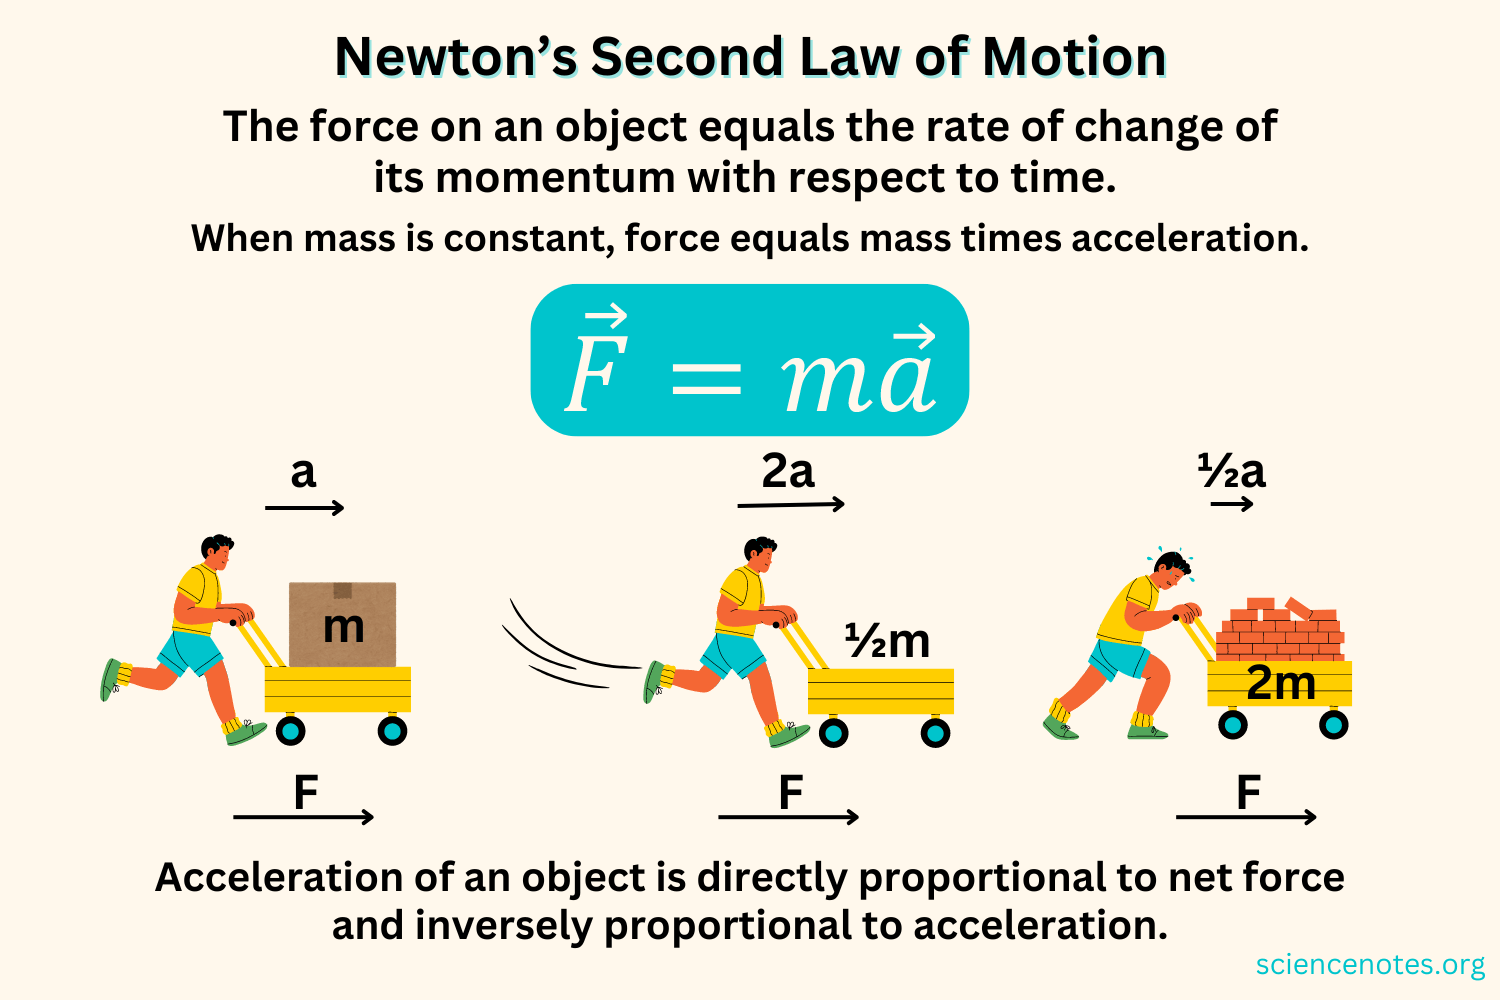
\includegraphics[width=0.8\textwidth]{Newtons-Second-Law-of-Motion.png}
    \caption{Illustration de la deuxième loi de Newton ($F = ma$) : influence de la masse sur la force requise pour une accélération donnée.}
    \label{fig:newton_law}
\end{figure}

\subsection{Les forces dissipatives : Résistance au roulement et traînée aérodynamique}

La masse n'agit pas seule. Elle amplifie les autres résistances au mouvement :
\begin{enumerate}
    \item \textbf{Résistance au roulement ($F_{rr}$) :} $F_{rr} = C_{rr} \cdot m \cdot g$. Plus un véhicule est lourd, plus le pneu se déforme sur la route, transformant l'énergie en chaleur dissipée inutilement.
    \item \textbf{Traînée aérodynamique :} Bien que liée à la forme aérodynamique ($C_x$), l'augmentation de la masse des véhicules modernes s'accompagne souvent d'une hausse de la surface frontale ($S$), augmentant la force de traînée $F_a = \frac{1}{2} \rho C_x S v^2$.
\end{enumerate}

% ============================================================
\section{La Chimie du Moteur : Quand le Poids devient Poison}
% ============================================================

\subsection{Le mécanisme de formation des \texorpdfstring{\ce{NOx}}{NOx}}

Pourquoi le poids génère-t-il des \ce{NOx} ? Pour déplacer un SUV lourd, le moteur doit fournir une pression de combustion plus élevée dans les cylindres. Cette pression élève la température de combustion. Au-delà de \SI{1400}{\celsius}, la molécule de diazote (\ce{N2}) atmosphérique se dissocie et réagit avec l'oxygène selon la réaction de Zeldovich :
\begin{equation}
    \ce{N2 + O -> NO + N} \qquad \text{puis} \qquad \ce{N + O2 -> NO + O}
\end{equation}
C'est le paradoxe fondamental : plus on cherche de la puissance pour compenser la masse, plus on crée des \ce{NOx} toxiques. Les systèmes SCR ajoutés pour traiter ces \ce{NOx} alourdissent encore le véhicule, créant un cercle vicieux entre masse, puissance et pollution.

\subsection{L'abrasion : le problème des véhicules électriques lourds}

L'abrasion des pneus et des freins représente aujourd'hui une part croissante des émissions de particules fines. Un véhicule électrique, bien que "zéro émission" à l'échappement, possède une masse élevée du fait de ses batteries (souvent 500 à 800 kg supplémentaires). Lors de chaque freinage, l'énergie cinétique --- proportionnelle à la masse (équation \ref{eq:ec}) --- doit être dissipée mécaniquement, arrachant des micro-particules de gomme et de métal. Ce phénomène peut rendre les émissions particulaires d'un SUV électrique comparables, voire supérieures, à celles d'une citadine thermique légère. Cela souligne que la réglementation actuelle, focalisée sur les émissions à l'échappement, sous-estime structurellement l'impact des véhicules lourds sur la qualité de l'air urbain.

% ============================================================
\section{Revue de Littérature et Approches Économétriques}
% ============================================================

Les sections précédentes ont établi les fondements physiques et réglementaires des émissions automobiles. Cette section recense et analyse les principaux travaux économétriques récents (2019--2024) qui ont cherché à quantifier ces déterminants à partir de données empiriques, afin d'ancrer notre propre analyse dans un cadre méthodologique éprouvé.

\subsection{Convergence des résultats : la masse et la puissance comme déterminants centraux}

L'ensemble de la littérature récente converge vers un constat central : les émissions de \ce{CO2} des véhicules sont avant tout déterminées par la masse et la puissance du moteur \cite{gonzalez2019, marrero2021, chatzipanagi2022}. Les élasticités estimées sont remarquablement cohérentes entre les études : une hausse de \SI{10}{\percent} de la masse du véhicule est associée à une augmentation de 6 à 8\% des émissions de \ce{CO2} (élasticité comprise entre 0,6 et 0,8), tandis que l'effet de la puissance, positif mais décroissant, suggère une relation non-linéaire. Ces résultats constituent le point de départ de notre propre spécification économétrique.

\subsection{Les modèles de panel dynamique}

\textbf{González et al. (2019)} et \textbf{Marrero et al. (2021)} s'inscrivent dans la famille des modèles de panel dynamique multi-pays. Ces auteurs exploitent des données de panel couvrant plusieurs décennies et de nombreux pays européens afin de modéliser les émissions moyennes de \ce{CO2} par kilomètre en fonction des caractéristiques agrégées du parc automobile. Leur approche repose sur la méthode des moments généralisés (GMM) de Arellano et Bond (1991), qui corrige les biais d'endogénéité liés à la présence de la variable dépendante retardée dans les équations.

Les variables explicatives incluent la masse moyenne du parc, la cylindrée moyenne, la part de véhicules diesel, l'âge moyen du parc, le revenu par habitant et des indicateurs de politiques environnementales. Leurs résultats confirment l'élasticité positive de la masse sur les émissions (0,6 à 0,8), et soulignent l'effet amplificateur de l'âge du parc : un parc plus ancien émet davantage, non seulement du fait d'une technologie moins efficiente, mais aussi en raison de la dégradation des systèmes de post-traitement.

\subsection{L'approche microéconométrique sur données de certification}

\textbf{Chatzipanagi et al. (2022)} adoptent une approche microéconométrique fondée sur les bases de données de certification européennes NEDC et WLTP, qui rassemblent les caractéristiques techniques de milliers de modèles homologués. À l'aide de modèles estimés par moindres carrés ordinaires (MCO) et de formes semi-logarithmiques, ils relient les émissions à la masse, à la puissance, à la résistance au roulement, au type de transmission et au rapport poids/puissance \cite{chatzipanagi2022}.

Leurs résultats confirment la forte corrélation entre masse et émissions (élasticité $\approx$ 0,7), et mettent en évidence un résultat méthodologique crucial pour notre étude : le passage du cycle NEDC au cycle WLTP conduit à une hausse moyenne d'environ \SI{12}{\percent} des émissions mesurées. Ce biais de mesure lié au changement de protocole d'homologation constitue une source d'hétérogénéité que toute analyse sur données de certification doit identifier et contrôler.

\subsection{Les modèles de parc dynamiques}

\textbf{Yan et al. (2024)} inscrivent leur travail dans la perspective des modèles de parc dynamiques. Leur objectif est de modéliser la relation entre la structure d'âge du parc automobile, la motorisation et les émissions globales. À l'aide d'un modèle de régression linéaire sur panel désagrégé intégrant des effets fixes temporels et nationaux, ils relient les émissions spécifiques à l'âge du véhicule, à son type de carburant (essence, diesel, hybride), à sa consommation spécifique et à son kilométrage moyen.

Leurs résultats indiquent que les émissions augmentent d'environ \SI{2.5}{\percent} par an de vieillissement du véhicule. Ce résultat est particulièrement pertinent dans le contexte français, où l'âge moyen du parc dépasse 10 ans : la stagnation du renouvellement, notamment pour les ménages à faibles revenus, constitue un frein structurel à la décarbonation.

\subsection{L'approche expérimentale sur données réelles}

\textbf{Rykała, Grzelak et Borucka (2024)} adoptent une approche expérimentale fondée sur des mesures directes d'émissions en conditions réelles, réalisées sur un échantillon de véhicules légers en Pologne. Ils combinent des régressions linéaires et logistiques pour estimer les déterminants des émissions mesurées en roulage réel, sans se limiter aux valeurs d'homologation \cite{rykala2024}.

Les variables explicatives incluent le poids, la cylindrée, la puissance, la vitesse moyenne et le type de carburant. Leurs résultats confirment l'impact positif de la masse et de la puissance sur les émissions (coefficients standardisés de +0,52 et +0,45 respectivement). Ils mettent en outre en évidence une relation non-linéaire entre vitesse et émissions, en forme de U : les émissions sont minimales entre 60 et 80 km/h, et augmentent fortement à basse vitesse (stop-and-go) comme à très haute vitesse. Les véhicules essence émettent en moyenne 10 à 15\% de plus de \ce{NOx} que leurs équivalents diesel en conditions réelles, un résultat qui nuance le discours ambiant défavorable au diesel.

\subsection{Limites méthodologiques et perspectives}

Ces études convergentes présentent néanmoins des limites communes que notre analyse s'efforce de dépasser. Premièrement, la mesure des émissions réelles reste difficile : les données d'homologation sous-estiment structurellement les émissions en usage réel, et les biais liés au changement de cycle (NEDC/WLTP) créent des discontinuités artificielles dans les séries temporelles. Deuxièmement, les fortes corrélations entre caractéristiques techniques des véhicules (masse, puissance, cylindrée) compliquent l'identification causale de l'effet propre de chaque variable. Troisièmement, les polluants locaux (\ce{NOx}, HC, particules fines) sont beaucoup moins souvent modélisés que le \ce{CO2}, créant un angle mort analytique que notre approche cherche précisément à combler.

La section empirique qui suit aborde ces limites en mobilisant les données de certification ADEME et en recourant à trois familles de modèles complémentaires : la régression OLS comme point de référence, le modèle Tobit pour traiter la censure à zéro des émissions des hybrides rechargeables, et l'Analyse de Frontière Stochastique (SFA) pour mesurer l'efficacité technique individuelle de chaque véhicule par rapport à la frontière des émissions minimales atteignables.

% ============================================================
\newpage
\begin{thebibliography}{99}

\bibitem{ue2019}
Union Européenne. (2019). \textit{Règlement (UE) 2019/631 fixant des normes de performance en matière d'émissions de \ce{CO2} pour les voitures particulières neuves}. Journal officiel de l'Union européenne.

\bibitem{gonzalez2019}
González, R., et al. (2019). \textit{Determinants of \ce{CO2} emissions from passenger cars in Europe: A dynamic panel analysis}.

\bibitem{marrero2021}
Marrero, G. A., et al. (2021). \textit{Weight, power and emissions: Econometric evidence from the European car market}.

\bibitem{chatzipanagi2022}
Chatzipanagi, A., et al. (2022). \textit{Evolution of European light-duty vehicle \ce{CO2} emissions: WLTP vs NEDC}. Transportation Research Part D.

\bibitem{rykala2024}
Rykała, J., Grzelak, M., et Borucka, A. (2024). \textit{Analysis of the determinants of \ce{CO2} emissions in real driving conditions}. Applied Sciences.

\bibitem{yan2024}
Yan, X., et al. (2024). \textit{Fleet age structure, fuel type and specific emissions: A dynamic panel approach}. Transportation Research Part D.

\bibitem{giec2023}
GIEC. (2023). \textit{Rapport de synthèse sur le changement climatique --- AR6}.

\bibitem{obfcm2024}
Commission Européenne. (2024). \textit{Real-world fuel and energy consumption of EU passenger cars --- OBFCM data publication 2021--2022}.

\end{thebibliography}

\end{document}